% Options for packages loaded elsewhere
\PassOptionsToPackage{unicode}{hyperref}
\PassOptionsToPackage{hyphens}{url}
\PassOptionsToPackage{dvipsnames,svgnames,x11names}{xcolor}
\PassOptionsToPackage{space}{xeCJK}
%
\documentclass[
  letterpaper,
  DIV=11,
  numbers=noendperiod]{scrartcl}

\usepackage{amsmath,amssymb}
\usepackage{iftex}
\ifPDFTeX
  \usepackage[T1]{fontenc}
  \usepackage[utf8]{inputenc}
  \usepackage{textcomp} % provide euro and other symbols
\else % if luatex or xetex
  \usepackage{unicode-math}
  \defaultfontfeatures{Scale=MatchLowercase}
  \defaultfontfeatures[\rmfamily]{Ligatures=TeX,Scale=1}
\fi
\usepackage{lmodern}
\ifPDFTeX\else  
    % xetex/luatex font selection
  \ifXeTeX
    \usepackage{xeCJK}
    \setCJKmainfont[BoldFont=STHeiti,ItalicFont=STKaiti]{STSong}
          \fi
  \ifLuaTeX
    \usepackage[]{luatexja-fontspec}
    \setmainjfont[BoldFont=STHeiti,ItalicFont=STKaiti]{STSong}
  \fi
\fi
% Use upquote if available, for straight quotes in verbatim environments
\IfFileExists{upquote.sty}{\usepackage{upquote}}{}
\IfFileExists{microtype.sty}{% use microtype if available
  \usepackage[]{microtype}
  \UseMicrotypeSet[protrusion]{basicmath} % disable protrusion for tt fonts
}{}
\makeatletter
\@ifundefined{KOMAClassName}{% if non-KOMA class
  \IfFileExists{parskip.sty}{%
    \usepackage{parskip}
  }{% else
    \setlength{\parindent}{0pt}
    \setlength{\parskip}{6pt plus 2pt minus 1pt}}
}{% if KOMA class
  \KOMAoptions{parskip=half}}
\makeatother
\usepackage{xcolor}
\setlength{\emergencystretch}{3em} % prevent overfull lines
\setcounter{secnumdepth}{-\maxdimen} % remove section numbering
% Make \paragraph and \subparagraph free-standing
\makeatletter
\ifx\paragraph\undefined\else
  \let\oldparagraph\paragraph
  \renewcommand{\paragraph}{
    \@ifstar
      \xxxParagraphStar
      \xxxParagraphNoStar
  }
  \newcommand{\xxxParagraphStar}[1]{\oldparagraph*{#1}\mbox{}}
  \newcommand{\xxxParagraphNoStar}[1]{\oldparagraph{#1}\mbox{}}
\fi
\ifx\subparagraph\undefined\else
  \let\oldsubparagraph\subparagraph
  \renewcommand{\subparagraph}{
    \@ifstar
      \xxxSubParagraphStar
      \xxxSubParagraphNoStar
  }
  \newcommand{\xxxSubParagraphStar}[1]{\oldsubparagraph*{#1}\mbox{}}
  \newcommand{\xxxSubParagraphNoStar}[1]{\oldsubparagraph{#1}\mbox{}}
\fi
\makeatother


\providecommand{\tightlist}{%
  \setlength{\itemsep}{0pt}\setlength{\parskip}{0pt}}\usepackage{longtable,booktabs,array}
\usepackage{calc} % for calculating minipage widths
% Correct order of tables after \paragraph or \subparagraph
\usepackage{etoolbox}
\makeatletter
\patchcmd\longtable{\par}{\if@noskipsec\mbox{}\fi\par}{}{}
\makeatother
% Allow footnotes in longtable head/foot
\IfFileExists{footnotehyper.sty}{\usepackage{footnotehyper}}{\usepackage{footnote}}
\makesavenoteenv{longtable}
\usepackage{graphicx}
\makeatletter
\def\maxwidth{\ifdim\Gin@nat@width>\linewidth\linewidth\else\Gin@nat@width\fi}
\def\maxheight{\ifdim\Gin@nat@height>\textheight\textheight\else\Gin@nat@height\fi}
\makeatother
% Scale images if necessary, so that they will not overflow the page
% margins by default, and it is still possible to overwrite the defaults
% using explicit options in \includegraphics[width, height, ...]{}
\setkeys{Gin}{width=\maxwidth,height=\maxheight,keepaspectratio}
% Set default figure placement to htbp
\makeatletter
\def\fps@figure{htbp}
\makeatother

\KOMAoption{captions}{tableheading}
\makeatletter
\@ifpackageloaded{caption}{}{\usepackage{caption}}
\AtBeginDocument{%
\ifdefined\contentsname
  \renewcommand*\contentsname{Table of contents}
\else
  \newcommand\contentsname{Table of contents}
\fi
\ifdefined\listfigurename
  \renewcommand*\listfigurename{List of Figures}
\else
  \newcommand\listfigurename{List of Figures}
\fi
\ifdefined\listtablename
  \renewcommand*\listtablename{List of Tables}
\else
  \newcommand\listtablename{List of Tables}
\fi
\ifdefined\figurename
  \renewcommand*\figurename{Figure}
\else
  \newcommand\figurename{Figure}
\fi
\ifdefined\tablename
  \renewcommand*\tablename{Table}
\else
  \newcommand\tablename{Table}
\fi
}
\@ifpackageloaded{float}{}{\usepackage{float}}
\floatstyle{ruled}
\@ifundefined{c@chapter}{\newfloat{codelisting}{h}{lop}}{\newfloat{codelisting}{h}{lop}[chapter]}
\floatname{codelisting}{Listing}
\newcommand*\listoflistings{\listof{codelisting}{List of Listings}}
\makeatother
\makeatletter
\makeatother
\makeatletter
\@ifpackageloaded{caption}{}{\usepackage{caption}}
\@ifpackageloaded{subcaption}{}{\usepackage{subcaption}}
\makeatother

\ifLuaTeX
  \usepackage{selnolig}  % disable illegal ligatures
\fi
\usepackage{bookmark}

\IfFileExists{xurl.sty}{\usepackage{xurl}}{} % add URL line breaks if available
\urlstyle{same} % disable monospaced font for URLs
\hypersetup{
  pdftitle={Introduction},
  colorlinks=true,
  linkcolor={blue},
  filecolor={Maroon},
  citecolor={Blue},
  urlcolor={Blue},
  pdfcreator={LaTeX via pandoc}}


\title{Introduction}
\author{}
\date{}

\begin{document}
\maketitle


\section{Introduction}\label{introduction}

How can college students find sustainability-focused companies? My
research project describes the process of designing a sustainable
shopping, saving, and investing companion. If used wisely, money can
help build communities of sustainable impact and helpo build closer
relationships with sustainability.

\subsection{Research Relevance}\label{research-relevance}

My research is timely in 2024 because of the convergence of the
following 5 major trending themes:

\begin{longtable}[]{@{}
  >{\raggedright\arraybackslash}p{(\columnwidth - 0\tabcolsep) * \real{1.0000}}@{}}
\caption{Current trends backing the relevance of this
research.}\tabularnewline
\toprule\noalign{}
\begin{minipage}[b]{\linewidth}\raggedright
Supernarratives
\end{minipage} \\
\midrule\noalign{}
\endfirsthead
\toprule\noalign{}
\begin{minipage}[b]{\linewidth}\raggedright
Supernarratives
\end{minipage} \\
\midrule\noalign{}
\endhead
\bottomrule\noalign{}
\endlastfoot
Increasing environmental degradation \\
Increasing interest in sustainability among young people \\
Intergenerational money transfer; in some countries relatively young
people have money \\
Increasing availability of sustainability tools such as ESG, B
Corporations, Green Bonds, etc, among metrics and instruments \\
Increasing availability and adoption of generative AI-based user
interfaces \\
\end{longtable}

\subsection{Research Background}\label{research-background}

I grew up reading science fiction books and their influence on my
outlook towards future possibilities continues until present day. In
particular, Star Trek has a portable device called a
\textbf{\emph{tricorder}} (fig.~1), which enables imaginary future
humans fix all kinds of problems from looking for minerals inside a cave
to scanning human bodies for medical information. I would love to have
such a device for consumer choices and financial decisions in order to
know what to buy and which businesses to do business with.

\begin{figure}[H]

{\centering 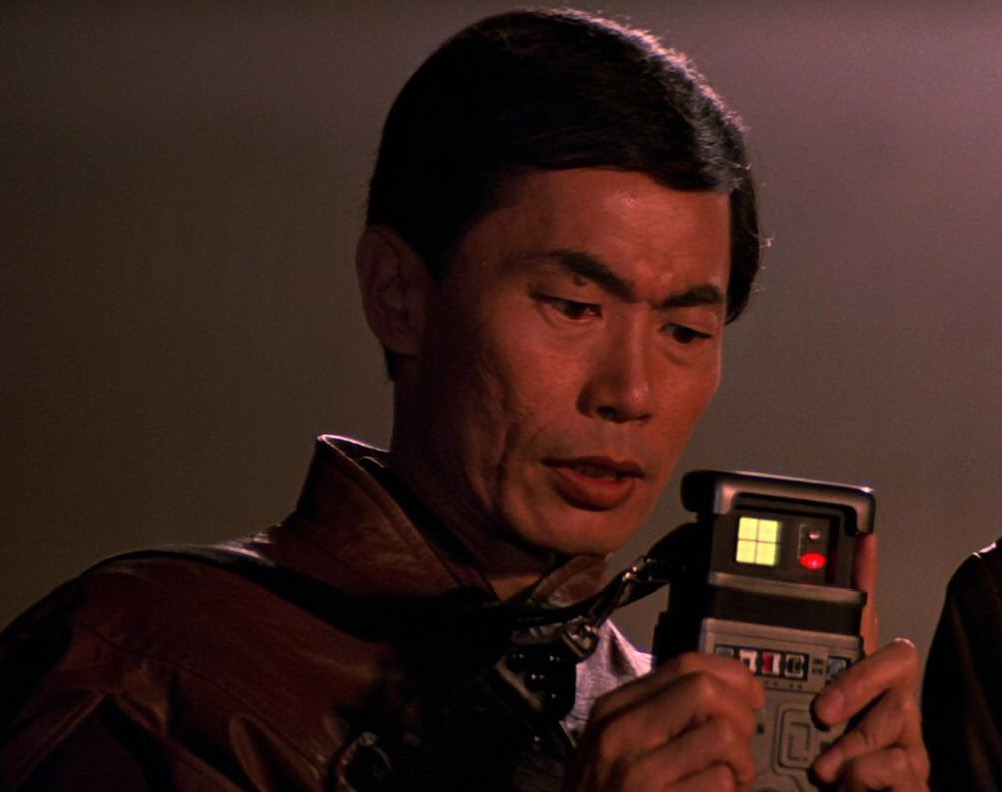
\includegraphics[width=0.5\textwidth,height=\textheight]{./images/tricorder.jpg}

}

\caption{Captain Sulu using a Tricorder (Star Trek) - Photo copyright by
Paramount Pictures}

\end{figure}%

\subsection{Research Motivation}\label{research-motivation}

Environmental issues are largely caused by production and manufacturing
processes of the companies that make the products we consume on a daily
basis. Without reliable and easily accessible data, it's difficult to
know which company is more sustainable than the other. We don't really
know what's green, unless we spend a lot of time looking at the numbers,
which may be costly to access (for example ESG reports are expensive).

AIs are already integral to many parts of our lives; this thesis was
partially written using Google's, Apple's, and OpenAIs voice recognition
software, allowing me to transcribe notes with the help of an AI
assistant. As a foreigner living in Taiwan, I've relied extensively on
AI assistants for many aspects of my life: to communicate, move around
efficiently, find food and services. Even when we don't realize it, AI
assistants helping us with many of our mundane tasks. When writing in
Chinese, Apple's text prediction algorithms translate pinyin to 漢字 and
show the most likely character based on my previous writing, Google's
maps find efficient and eco-friendly routes and recommend places to eat
and ChatGPT provides statistically probable advice from the sum of human
knowledge. While it takes incredibly complex computational algorithms to
achieve all this in the background, it's become so commonplace, we don't
even think about it. From this point of view, another AI assistant to
help humans with choosing more eco-friendly businesses to show, save,
and invest doesn't sound so much of a stretch.

\subsection{Research Objective}\label{research-objective}

The study presents an AI companion design which seeks to help people
build relationships with sustainability-focused companies. The major
contribution of this study is an interactive artefact (a prototype)
informed by design research.

\subsection{Research Demographics}\label{research-demographics}

My research targets respondents according to the following criteria.

\begin{longtable}[]{@{}ll@{}}
\toprule\noalign{}
Criteria & \\
\midrule\noalign{}
\endhead
\bottomrule\noalign{}
\endlastfoot
Location & Taiwan \\
Population & College Students \\
Count & 700 \\
\end{longtable}

Interviews with experts (finance, design, sustainability).

\begin{longtable}[]{@{}ll@{}}
\toprule\noalign{}
Criteria & \\
\midrule\noalign{}
\endhead
\bottomrule\noalign{}
\endlastfoot
Location & Global \\
Population & Experts \\
Count & 5 \\
\end{longtable}

\subsection{Research Questions}\label{research-questions}

My research aims to answer the following questions.

\begin{longtable}[]{@{}
  >{\raggedright\arraybackslash}p{(\columnwidth - 4\tabcolsep) * \real{0.2639}}
  >{\raggedright\arraybackslash}p{(\columnwidth - 4\tabcolsep) * \real{0.4167}}
  >{\raggedright\arraybackslash}p{(\columnwidth - 4\tabcolsep) * \real{0.3194}}@{}}
\caption{Table of research questions.}\tabularnewline
\toprule\noalign{}
\begin{minipage}[b]{\linewidth}\raggedright
№
\end{minipage} & \begin{minipage}[b]{\linewidth}\raggedright
Question
\end{minipage} & \begin{minipage}[b]{\linewidth}\raggedright
Methods
\end{minipage} \\
\midrule\noalign{}
\endfirsthead
\toprule\noalign{}
\begin{minipage}[b]{\linewidth}\raggedright
№
\end{minipage} & \begin{minipage}[b]{\linewidth}\raggedright
Question
\end{minipage} & \begin{minipage}[b]{\linewidth}\raggedright
Methods
\end{minipage} \\
\midrule\noalign{}
\endhead
\bottomrule\noalign{}
\endlastfoot
1 & In general, what are some trends in how sustainability interacts
with AI, design, and finance? & Literature Review \\
2 & What are some fundamental requirements for designing an AI-assistant
aiming to help college students participate in sustainable financial
activism? & Literature Review and Expert Interviews \\
3 & What features do college students prioritize and what questions
would they prefer to ask a sustainability AI assistant? & Survey
(Taiwanese College Student) \\
\end{longtable}




\end{document}
